
\section{Lexical Semantics}

\begin{frame}{Lexical Semantics}

\begin{itemize}
\item Lexical semantics is concerned with the identification and
  representation of the semantics of lexical items
\item If we are to identify the semantics of lexical items, we have to
  be prepared for the eventuality of a given word having 
  multiple interpretations
  \begin{itemize}
  \item \txx{Polysemy}: having multiple meanings
  \item \txx{Monosemy}: having only one meaning
  \end{itemize}
\item \txx{Homonyms} are words with two unrelated meanings:
  \begin{itemize}
  \item \txx{homographs}: same spelling 
    \\ \eng{bow} vs \eng{bow}; \eng{keep} vs \eng{keep}
  \item \txx{homophones}: same pronunciation
     \\ \eng{right} vs \eng{write}; \eng{keep} vs \eng{keep}
  \end{itemize}

\end{itemize}





\end{frame}

% \begin{frame}{Polysemy}

% \MyLogo{\citet{Cruse:1986,Hirst:1987,_Ravin:Leacock:2000,Pustejovsky:1995}}

% \begin{itemize}
% \item \textbf{Polysemy} = the condition of a single lexical item having
%   multiple meanings
% \item Polysemy vs.\ homonymy (cf.\ \eng{bank} vs.\ \eng{bass})
% \item Polysemy vs.\ indeterminacy (cf.\ \eng{father} vs.\ \eng{uncle})
% \item Regular/logical vs.\ irregular polysemy (cf.\ \eng{ash})
% \item Regular vs.\ complementary polysemy (cf.\ \eng{door} vs.\ \eng{farm})
% \end{itemize}

%\end{frame}

\begin{frame}{Distinguishing Polysemes}

%The polysemy of a word can be tested by a variety of means, including:
\begin{itemize}
\item \txx{Antagonism}: can the word be used in a sentence with
  multiple \underline{competing} interpretations that are incompatible? \\[1ex]
  \eng{Kim can't  bear children}
  \begin{itemize}
  \item Cannot have children
  \item Doesn't like children
  \end{itemize}
\item \txx{Zeugma}: can the word be used in a context where multiple
  \underline{competing} interpretations are simultaneously evoked? \\[1ex]
  \eng{Kim and her visa expired}
    \begin{itemize}
    \item died
    \item ran out
    \end{itemize}
 \eng{Hitmen were quite expensive, so she decided to take out a loan and her husband.} \task
  \item  \txx{Paraphrase/Translation}: Is there more than one (clearly different) way to paraphrase/translate the word.
  \end{itemize}
\end{frame}

\begin{frame}{Necessary and Sufficient Conditions}

\begin{itemize}
\item Can we define words in terms of \txx{conditions}?
  \begin{itemize}
  \item \lex{zebra}
    \begin{itemize}
    \item quadruped
    \item animal \txx{redundant}
    \item black and white striped
    \item herbivore
    \end{itemize}
  \end{itemize}
\item These are \txx{intrinsic}, \txx{generic} properties
  
  \begin{itemize}
  \item An albino zebra with three legs is still a zebra
  \end{itemize}
\item Can we use words even if we don't know their properties?
  \begin{itemize}
  \item \lex{Kway Teow}
  \end{itemize}
\item We seem to be ok with fairly vague definitions
  \begin{taskb}
  \begin{itemize}
  \item What is a \lex{dog-cart}? 
  \item What is a \lex{grass snake}?
  \item What is a \lex{swamp adder}?
  \end{itemize}
\end{taskb}
\end{itemize}

\end{frame}

\begin{frame}{Words/Concepts are related in many ways}

We can also look at words (or more properly senses) in terms of their
relations to other words.

\begin{itemize}
\item \txx{Hyponymy/Hypernymy}
\item \txx{Synonymy}
\item \txx{Antonymy} (Opposites)
\item \txx{Meronymy}
    \begin{itemize}
    \item \txx{Member-Collection}
    \item \txx{Portion-Mass}
    \item \txx{Element-Substance}
    \end{itemize}
  \item \txx{Domain} (lexical field)
\end{itemize}




\end{frame}

\begin{frame}{Hypernymy and Hyponymy}

\begin{itemize}
\item \txx{Hyponymy}: X is a hyponym of Y iff
  $f(X)$ entails $f(Y)$ but $f(Y)$ does not entail $f(X)$ (for all or most $f$):
  \begin{quote}
    \eng{Kim has a pet \underline{dog} $\vDash$  Kim has a pet \underline{animal}}\\
    \eng{Kim has a pet \underline{animal} $\not\vDash$  Kim has a pet \underline{dog}}
  \end{quote}
  N.B.\ complications with universal quantifiers and negation:
  \begin{quote}
    \eng{Kim likes all \underline{animals} $\vDash$  Kim likes all \underline{dogs}}\\
    \eng{Kim likes all \underline{dogs} $\not\vDash$  Kim likes all \underline{animals}}
  \end{quote}
\item \txx{Hypernymy}: Y is a hypernym of X iff X is a hyponym of Y
\item Can a word have multiple hypernyms?
  \begin{exe}
    \ex \lex{tank$_1$} $\subset$ \lex{military\_vehicle$_1$}; $\subset$ \lex{tracked\_vehicle}$_1$; 
    $\subset$ \lex{armored\_vehicle$_1$}; ? $\subset$ \lex{weapon$_1$}
  \end{exe}
\end{itemize}

\end{frame}

\begin{frame}{What is \txx{entailment}}
\begin{quote}
  \txx{Entailment} ($\vDash$): A sentence $p$ entails a sentence $q$ when the
  truth of the first ($p$) guarantees the truth of the second ($q$),
  and the falsity of the second ($q$) guarantees the falsity of the
  first ($p$).
\end{quote}
\end{frame}

\begin{frame}{Properties of hypernymy/hyponymy}
  \begin{itemize}\addtolength{\itemsep}{-0.5ex}
  \item Asymmetric; applies at the sense level
  \item applies only to lexical items of the same word class
  \item Transitive: \lex{dog$_1$} $\subset$ \lex{mammal$_1$} $\subset$ \lex{animal$_1$}
  \item Not all nodes are lexicalized; can be multiple \\[2ex]
    \begin{tabular}{llll}
      neutral (Hyper) & male & female & child \\ \hline
%      pig & hog & sow & piglet\\
      \lex{sheep} & \lex{ram} & \lex{ewe} & \lex{lamb}\\
      \lex{cow} & \lex{bull} & \lex{\ul{cow}} & \lex{calf} \\
      \lex{goose} & \lex{gander} & \lex{\ul{goose}} & \lex{gosling}  \\
      \lex{horse} & \lex{stallion} & \lex{mare} & \lex{foal:colt/filly} \\
      \lex{dog} &  \lex{\ul{dog}} &  \lex{bitch} &\lex{puppy} \\
      \lex{snake} & \lex{\ul{snake}}& \lex{\ul{snake}}& \lex{\ul{snake}}\\
    \end{tabular}
    \begin{taskb}
      Can you do this for \lex{pig}, \lex{cat} or \lex{chicken}?
    \end{taskb}
   \begin{taskb}
 Can you give an example of this in another language?
\end{taskb}

  \end{itemize}
\end{frame}

\begin{frame}[allowframebreaks]{Language Change and Auto-hyponyms}

\begin{itemize}%\addtolength{\itemsep}{-1ex}
\item The meanings of words change over time
  \begin{itemize}
  \item \lex{guitar} --- ``a stringed instrument usually having six
    strings'': originally these all used the body to make sound
    
\item We then get \lex{electric guitar} --- ``a guitar with a built-in
  pickup or pickups which convert string vibrations into electrical
  signals for amplification''
\item To refer to non-electric guitars we get a new coining
  \lex{acoustic guitar} -- ``a guitar that does not require electrical
  amplification'': which used to just be guitar
\end{itemize}
  \item \lex{guitar} is now a hypernym of them both and can refer to
    either
 \item we can also refer to the prototypical guitar (acoustic) using
   reduplication
   \\ \eng{What kind of guitar do you play?}  \eng{\ul{Guitar guitar}}

\framebreak
  
\item Sometimes this practice becomes politically charged, although
  linguistically it is unremarkable
  \begin{itemize}
  \item \lex{woman} ``an adult female person''
  \item \lex{trans woman} ``a person who identifies as a woman but was assigned male at birth''
  \item \lex{cis woman}  ``a person who identifies as a woman and was assigned female at birth''
  \end{itemize}
  \end{itemize}
  \begin{taskb}
    Can you give other examples of this in English or other languages?
  \end{taskb}

  % milk, dairy milk
%mother, surrogate mother, stepmother, foster mother, god mother,
%adoptive mother, biological mother

% rice, cooked rice, chocolate rice, wild rice, brown rice
% 
\end{frame}

\begin{frame}{Synonymy}

\begin{itemize}
\item \txx{Propositional synonymy}: X is a propositional synonym of Y if
  \begin{itemize}
  \item   (i) X and Y are syntactically identical,
  \item (ii) substitution of Y  for X in a declarative sentence doesn't change its truth conditions
  \end{itemize}
  e.g., \lex{violin} and \lex{fiddle}
\item Why propositional synonymy is over-restrictive:
  \begin{itemize}
  \item syntactic identity (cf.\ \lex{eat} and \lex{devour})
  \item collocations (cf.\ \lex{cemetery} and \lex{graveyard})
  \item gradability (cf.\ \lex{sofa}/\lex{settee} vs.\ \lex{boundary/frontier})
  \end{itemize}
\end{itemize}
\end{frame}

\begin{frame}{Near Synonymy}
\begin{itemize}
\item Near synonyms are substitutable in \textbf{some/most} rather than \textbf{all} contexts
\item Synonymy via semantics: synonyms share ``common traits'' or
  attributional overlap, walking the fine line between ``necessary
  resemblances'' and ``permissible differences'':
  \begin{quote}
      \lex{grain} vs. \lex{granule};  \lex{green} vs.\ \lex{purple}; \lex{alsation} vs. \lex{spaniel}
  \end{quote}
\item Permissible differentiation via \textbf{clarification}.
  \begin{quote}
    \eng{Here is a \underline{grain}, or \underline{granule}, of the substance.}\\
    \eng{* The cover is \underline{green}, \{or, that is to say\} \underline{purple}.}
    \\   \eng{* He likes alsations, in other words, \underline{spaniels}}
    
  \end{quote}
%   and \textbf{contrast}:
%   \begin{quote}
%     \eng{Here is a \underline{grain} or, more exactly, \underline{granule}}\\
%     \eng{* He likes alsations, or more exactly, \underline{spaniels}}
%   \end{quote}
%
\end{itemize}
\end{frame}

\begin{frame}{Properties of synonymy}

  \begin{itemize}
  \item Symmetric
  \item traditionally applies only to lexical items of the same word class
    \\ but pairs like \lex{can} vs \lex{be able to} suggest otherwise
  \item applied at the sense level
  \item $\approx$ converse of polysemy
  \end{itemize}


\end{frame}


\begin{frame}{Semantic Relations as Graphs ($p \subset q$ and $p \sim q$)}
\MyLogo{\textit{Yes it is}}

\begin{tabular}{cc}
$p \subset q$ \iz{hypernym}  & $p \sim q$ \iz{synonym} \\[2ex] 
\scalebox{2}{
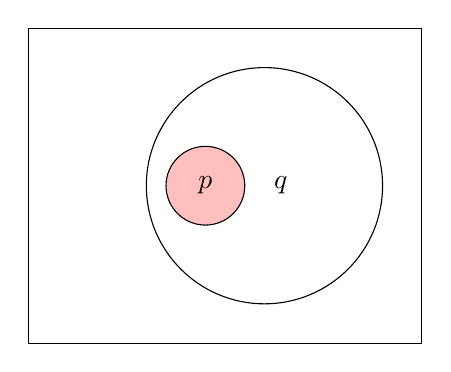
\begin{tikzpicture}
\filldraw[fill=white] (-2,-2) rectangle (3,2);
\scope % A \vee B
%\clip (0,0) circle (1);
\fill[pink] (0.25,0) circle (0.5);
%\fill[white] (0,0) circle (1);
\endscope
\draw (0.25,0) circle (0.5) node [text=black] {$p$}
      (1,0) circle (1.5) node [text=black,right] {$q$};
% outline
\end{tikzpicture}}
&
\scalebox{2}{
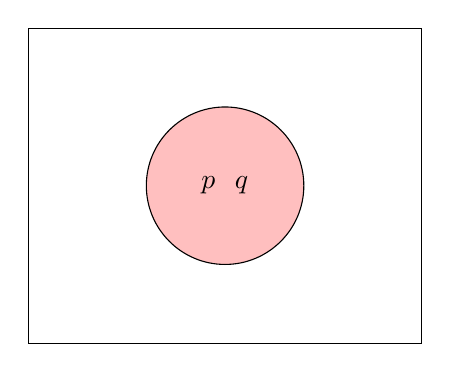
\begin{tikzpicture}
\filldraw[fill=white] (-2,-2) rectangle (3,2);
\scope % A \vee B
%\clip (0,0) circle (1);
%\fill[pink] (1,0) circle (1);
\fill[pink] (0.5,0) circle (1);
\endscope
\draw (0.5,0) circle (1) node [text=black,left] {$p$}
      (0.5,0) circle (1) node [text=black,right] {$q$};
% outline
\end{tikzpicture}}

\end{tabular}
\end{frame}

\begin{frame}[allowframebreaks]{Antonymy (opposites)}

%\MyLogo{\citet{Cruse:1986,Miller:1990}}

\begin{itemize}
\item \txx{Simple antonyms}: the negative of one implies the positive of the other.
  \begin{exe}
    \ex \eng{dead/alive}
    \ex \eng{pass/fail}
  \end{exe}
\item \txx{Gradable Antonyms}: points  along a scale
  \begin{exe}
    \ex \eng{boiling/hot/warm/tepid/cool/cold/freezing}
    \ex \eng{fascinating/interesting/dull/boring}
  \end{exe}
\item \txx{Reverses}: reverse the direction of a motion
  \begin{exe}
    \ex \eng{ascend/descend}
    \ex \eng{up/down; right/left}
  \end{exe}
\framebreak
\item \txx{Converses}: the same act from different points of view
  \begin{exe}
    \ex \eng{above/below; right/left}
    \ex \eng{employer/employee}
  \end{exe}
  (Slightly non-standard usage by Saeed)
\item \txx{Taxonomic Sisters}: children of the same (grand)parent
  \begin{exe}
    \ex \eng{Monday/Tuesday/\ldots{}/Sunday}
    \\ \textnormal{in WordNet:} \lex{day of the week} $\supset$ \lex{weekday}, \lex{weekend}
    \ex \eng{LMS/English/Chinese/\ldots}
    \\  \textnormal{Context dependent}
  \end{exe}
\end{itemize}
\end{frame}

\begin{frame}{Meronymy}

\begin{itemize}
\item \txx{Meronomy} refers to the part-whole relation
  \begin{itemize}
  \item \txx{meronym} is the part
  \item \txx{holonym} is the whole
  \end{itemize}
\begin{forest}
  [car
    [wheel
      [tire]
      [rim]
    ]
    [engine
      [piston]
      [valve]
    ]
    [door]
    [steering wheel]
  ]
\end{forest}
\item It is not always transitive:
  
\begin{forest}
  [shirt
    [button
      [button hole]
    ]
  ]
\end{forest}

We don't normally say that a \lex{button hole} is part of a \lex{shirt}.
\end{itemize}
\end{frame}

\begin{frame}{Member-Collection}

\begin{itemize}
\item The relation between a collection and one of the units that makes it up
  \begin{exe}
    \ex \eng{tree--forest}
    \ex \eng{sheep--flock}
    \ex \eng{fish--school}
    \ex \eng{book--library}
    \ex \eng{member--band}
    \ex \eng{musician--orchestra}
    \ex \eng{student--class}
  \end{exe}
\end{itemize}
\end{frame}

\begin{frame}{Portion-Mass}

\begin{itemize}
\item The relation between a mass noun and a typical unit of measurement
  \begin{exe}
    \ex \eng{drop--liquid}
    \ex \eng{grain--sand/salt/truth}
    \ex \eng{sheet/ream--paper}
    \ex \eng{lump--coal (or just about anything)}
    \ex \eng{strand--hair}
    \ex \eng{rasher--bacon}
  \end{exe}
\item Similar to classifiers in many ways, e.g. in Malay
  \begin{exe}
    \ex \eng[tail]{ekor}--\eng{animal}
    \ex \eng[human]{orang}--\eng{person}
  \end{exe}
\end{itemize}
\end{frame}

\begin{frame}{Domain (lexical field)}
\MyLogo{Examples from WordNet 3.0}
The domain in which a word is typically used with this meaning.

\begin{exe}
  \ex \lex{driver$_1$} --- the operator of a motor vehicle
  \ex \lex{driver$_2$} --- someone who drives animals that pull a vehicle
  \ex \lex{driver$_3$} --- a golfer who hits the golf ball with a driver [\con{golf}] 
  \ex \lex{driver$_4$} --- ($\simeq$ device driver) a program that determines how a computer will communicate with a peripheral device [\con{computer science}] 
  \ex \lex{driver$_5$} --- ($\simeq$ number one wood) a golf club (a wood) with a near vertical face that is used for hitting long shots from the tee [\con{golf}] 
\end{exe}

Some \con{golf} terms: \lex{approach$_9$}, \lex{approach shot$_1$}, \lex{golf course$_1$}, \lex{links course$_1$}, \lex{wedge$_5$}, \lex{tee$_1$}, \lex{scratch$_9$}, \lex{putt$_1$}, \lex{slice$_1$}, \lex{hook$_1$}

       % TOPIC TERM->(adj) dormie#1, dormy#1
       % TOPIC TERM->(adj) greenside#1
       % TOPIC TERM->(noun) approach#9, approach shot#1
       % TOPIC TERM->(noun) chip#8, chip shot#1
       % TOPIC TERM->(noun) driving iron#1, one iron#1
       % TOPIC TERM->(noun) golf-club head#1, club head#1, club-head#1, clubhead#1
       % TOPIC TERM->(noun) golf course#1, links course#1
       % TOPIC TERM->(noun) golf equipment#1
       % TOPIC TERM->(noun) golf range#1, driving range#1
       % TOPIC TERM->(noun) heel#6
       % TOPIC TERM->(noun) plus fours#1
       % TOPIC TERM->(noun) toe#4
       % TOPIC TERM->(noun) wedge#5
       % TOPIC TERM->(noun) whip#4
       % TOPIC TERM->(noun) loft#3
       % TOPIC TERM->(noun) address#7
       % TOPIC TERM->(noun) scratch#9
       % TOPIC TERM->(noun) card#8, scorecard#1
       % TOPIC TERM->(noun) apron#2
       % TOPIC TERM->(noun) divot#2
       % TOPIC TERM->(noun) divot#1
       % TOPIC TERM->(noun) greenskeeper#1
       % TOPIC TERM->(noun) medalist#2, medallist#2, medal winner#1
       % TOPIC TERM->(noun) stroke#6
       % TOPIC TERM->(noun) birdie#1
       % TOPIC TERM->(noun) bogey#2
       % TOPIC TERM->(noun) double-bogey#1
       % TOPIC TERM->(noun) eagle#2
       % TOPIC TERM->(noun) double eagle#1
       % TOPIC TERM->(noun) par#1
       % TOPIC TERM->(verb) address#10
       % TOPIC TERM->(verb) tee off#1
       % TOPIC TERM->(verb) par#1
       % TOPIC TERM->(verb) ace#3
       % TOPIC TERM->(verb) caddie#1, caddy#1
       % TOPIC TERM->(verb) eagle#2
       % TOPIC TERM->(verb) hole up#2
       % TOPIC TERM->(verb) carry#36
       % TOPIC TERM->(verb) toe#4
       % TOPIC TERM->(verb) shank#1
       % TOPIC TERM->(verb) putt#1
       % TOPIC TERM->(verb) putt#2
       % TOPIC TERM->(verb) heel#4
       % TOPIC TERM->(verb) toe#3
       % TOPIC TERM->(verb) drive#17
       % TOPIC TERM->(verb) hole#1, hole out#1
       % TOPIC TERM->(verb) slice#2
       % TOPIC TERM->(verb) hook#4
       % TOPIC TERM->(verb) sclaff#2
       % TOPIC TERM->(verb) sclaff#1
       % TOPIC TERM->(verb) tee#1, tee up#2
       % TOPIC TERM->(verb) chip#3
       % TOPIC TERM->(verb) birdie#1
       % TOPIC TERM->(verb) eagle#1, double birdie#1
       % TOPIC TERM->(verb) double bogey#1
       % TOPIC TERM->(verb) bogey#1

\end{frame}

\begin{frame}{And More}
\MyLogo{}
\begin{itemize}
\item There are many, many more lexical relations advocated by various
  theories including:
  \begin{itemize}
  \item Troponymy/hypernymy (cf.\ \eng{walk} vs.\ \eng{lollop}) 
    ``way of doing something''
  \item Entailment (cf.\ \eng{snore} vs.\ \eng{sleep}) ``if you do one thing, you must be doing the other''
  \item Operator (cf.\ \eng{question} vs.\ \eng{ask})
    ``the thing you do by doing something''
  \item Magnifier (cf.\ \eng{wound} vs. \eng{badly})
    ``intensifier, diminisher''
  \item Usage (cf.\ \eng{strong-willed} vs. \eng{pig-headed} ``stubborn'')
    \\ \eng{pig-headed} is \txx{pejorative}
%  \item[] $\vdots$
  \end{itemize}
\end{itemize}
% \section{Sentence Types}

\end{frame}

